\documentclass[11pt, english]{article}
\usepackage{graphicx}
\usepackage[colorlinks=true, linkcolor=blue]{hyperref}
\usepackage[english]{babel}
\selectlanguage{english}
\usepackage[utf8]{inputenc}
\usepackage[svgnames]{xcolor}



\usepackage{listings}
\usepackage{afterpage}
\pagestyle{plain}

\definecolor{dkgreen}{rgb}{0,0.6,0}
\definecolor{gray}{rgb}{0.5,0.5,0.5}
\definecolor{mauve}{rgb}{0.58,0,0.82}

%\lstset{language=R,
%    basicstyle=\small\ttfamily,
%   stringstyle=\color{DarkGreen},
%    otherkeywords={0,1,2,3,4,5,6,7,8,9},
%    morekeywords={TRUE,FALSE},
%    deletekeywords={data,frame,length,as,character},
%    keywordstyle=\color{blue},
%    commentstyle=\color{DarkGreen},
%}

\lstset{frame=tb,
language=R,
aboveskip=3mm,
belowskip=3mm,
showstringspaces=false,
columns=flexible,
numbers=none,
keywordstyle=\color{blue},
numberstyle=\tiny\color{gray},
commentstyle=\color{dkgreen},
stringstyle=\color{mauve},
breaklines=true,
breakatwhitespace=true,
tabsize=3
}

\usepackage{here}


\textheight=21cm
\textwidth=17cm
%\topmargin=-1cm
\oddsidemargin=0cm
\parindent=0mm
\pagestyle{plain}

%%%%%%%%%%%%%%%%%%%%%%%%%%
% La siguiente instrucción pone el curso automáticamente%
%%%%%%%%%%%%%%%%%%%%%%%%%%

\usepackage{color}
\usepackage{ragged2e}

\global\let\date\relax
\newcounter{unomenos}
\setcounter{unomenos}{\number\year}
\addtocounter{unomenos}{-1}
\stepcounter{unomenos}


\begin{document}

\begin{titlepage}

\begin{center}
\vspace*{-1in}
\begin{figure}[htb]
\begin{center}

\end{center}
\end{figure}

\begin{large}
\textbf{LOG ME}\\
\end{large}
\vspace*{0.2in}
\begin{Large}

\end{Large}
\vspace*{0.3in}
\begin{large}
\\
\end{large}
\vspace*{0.3in}
\rule{80mm}{0.1mm}\\
\vspace*{0.1in}
\begin{large}
Made by: \\
Athira Nair K\\
\end{large}

\end{center}
\end{titlepage}

\newcommand{\CC}{C\nolinebreak\hspace{-.05em}\raisebox{.4ex}{\tiny\bf +}\nolinebreak\hspace{-.10em}\raisebox{.4ex}{\tiny\bf +}}
\def\CC{{C\nolinebreak[4]\hspace{-.05em}\raisebox{.4ex}{\tiny\bf ++}}}

\tableofcontents
\newpage
\section{Introduction}
\newline
This paper gives an overview of a login application, Log-Me helps the user to login to his/her private page,  Register if he/she is a new user. And it gives special consideration regarding security. Password checking, with the existing one present in the database. In case if both of the passwords matches, confirms the user to log in. Later, a page displaying Hello username will be shown.

\subsection{Scope}
\newline
Log-Me is a mini web application which helps a user, to begin with Login if he/she is a current user or register if he is a new user. Registration has been made more secure by keeping a key bound for passwords, certain common passwords and easily typed ones like qwerty,123 and user names are unacceptable. Email is sent to the user via mail servers to log in.
\newline
If these procedures go on fine, a person is directed to a page displaying Hello with a username. Log-Me can be used as a platform by most of the apps to create their login feature. It follows a secured format in user login.
\subsection{Definition}
\newline
\item Services : Functionalities offered by application.
\item Validation: Checks validity of user.
\item Update: Adding new information and changing previous one.
\item Push notifications: Messages that are received in the mail.


\subsection{Acronyms}
\newline
\item DD: Design Documentation
\item API: Application Program interface
\item DBMS: Database Management System.


\subsection{Document Structure}
\item Chapter1: Introduction
\item Chapter2: Architectural  Design
\item Chapter3: User Interface Design
\item Chapter4: Requirement Tractability
\item Chapter5: Implementation and Test plan
\item Chapter6: Effort Spent
\item Chapter7: References

\section{Architectural Design}
\newline
\subsection{Overview}
\newline
The whole project is divided into 5 classes:
\newline
\item\textbf{Admin:}
\newline
\newline Handles all the works and has the power to remove,add user.
\newline
\item\textbf{Login class:}
\item\item User is asked to enter his username and password to log in. Hence two attributes used here are User Id and password.
\item\item If entered details are incorrect(using validate login method), the user has accessibility to reset the password. 
\item\item Sign up is meant for a new user to login.
\item\item Another option is present to reset the password, where the user is asked to enter a new password and methods like delete changed password and add new password are included. Sign up and reset password is connected with the login page.
\newline
\item\textbf{Sign up:}
\item\item Here attributes like Username, password is used.
\item\item Methods like a register() to provide a link to the database to create a new token. When a user is registered, in the database the email_confirmed column set to False.
\item\item An email is concerned with a unique URL and each URL with a token.
\newline
\item\textbf{Reset password:}
\item\item A request to reset for a given account's email is sent.
\item\item When the user clicks the link, checks which email to confirm and sets email_confirmed column to True. This is the functionality of valid_mail().
\item\item Later the password of the user is changed in password column and the old one is deleted.
\item\item Here API fetching is used to provide login link to the user to his G-Mail/outlook mail.
\newline
\item\textbf{Display:}
\newline
\newline Displays with username via gethello() method.

\subsection{Class Diagram}

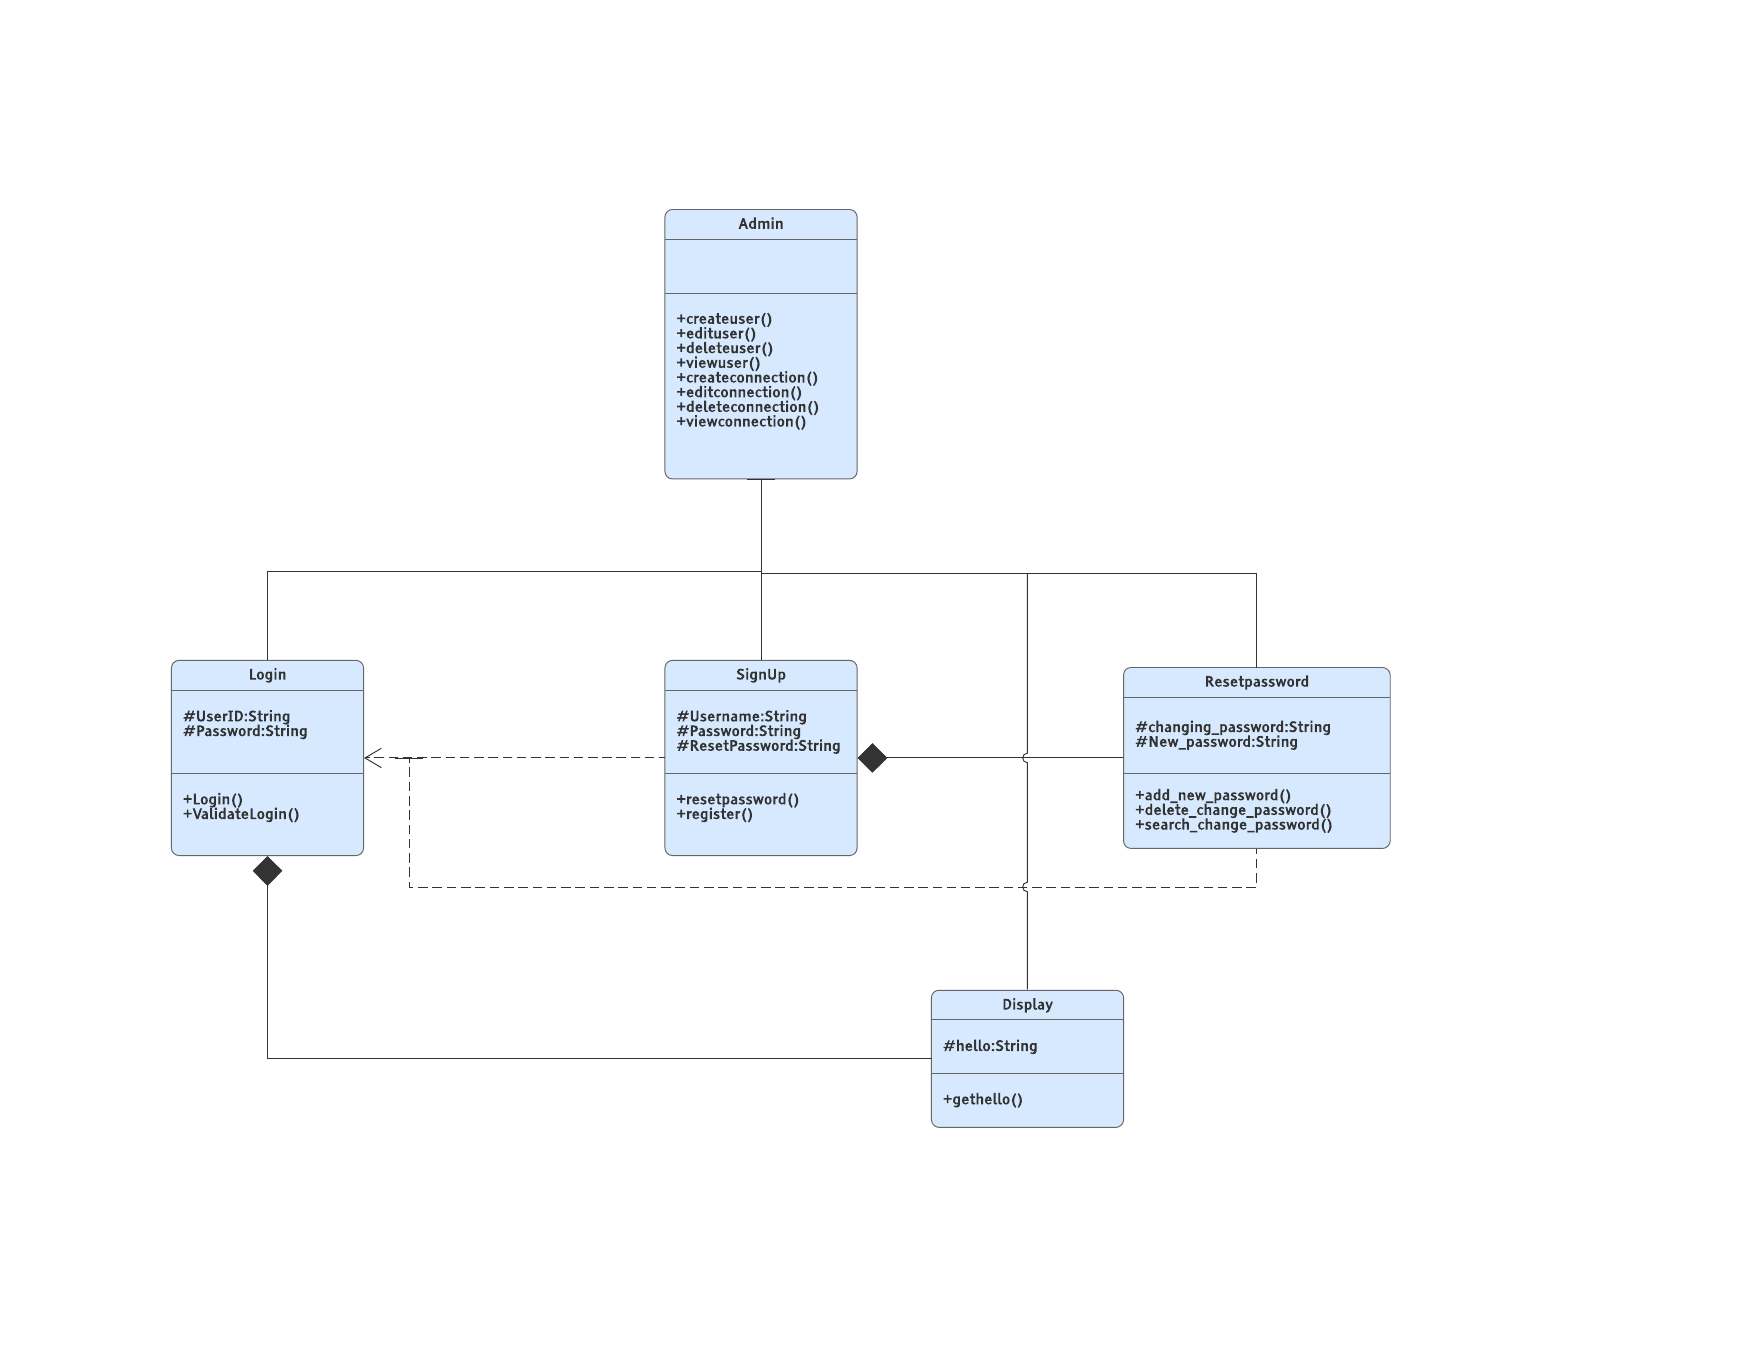
\includegraphics[width=200mm,scale=5.0]{ClassDiagram.png}

\subsection{Flow Chart}
\begin{center}
\newline
\newline
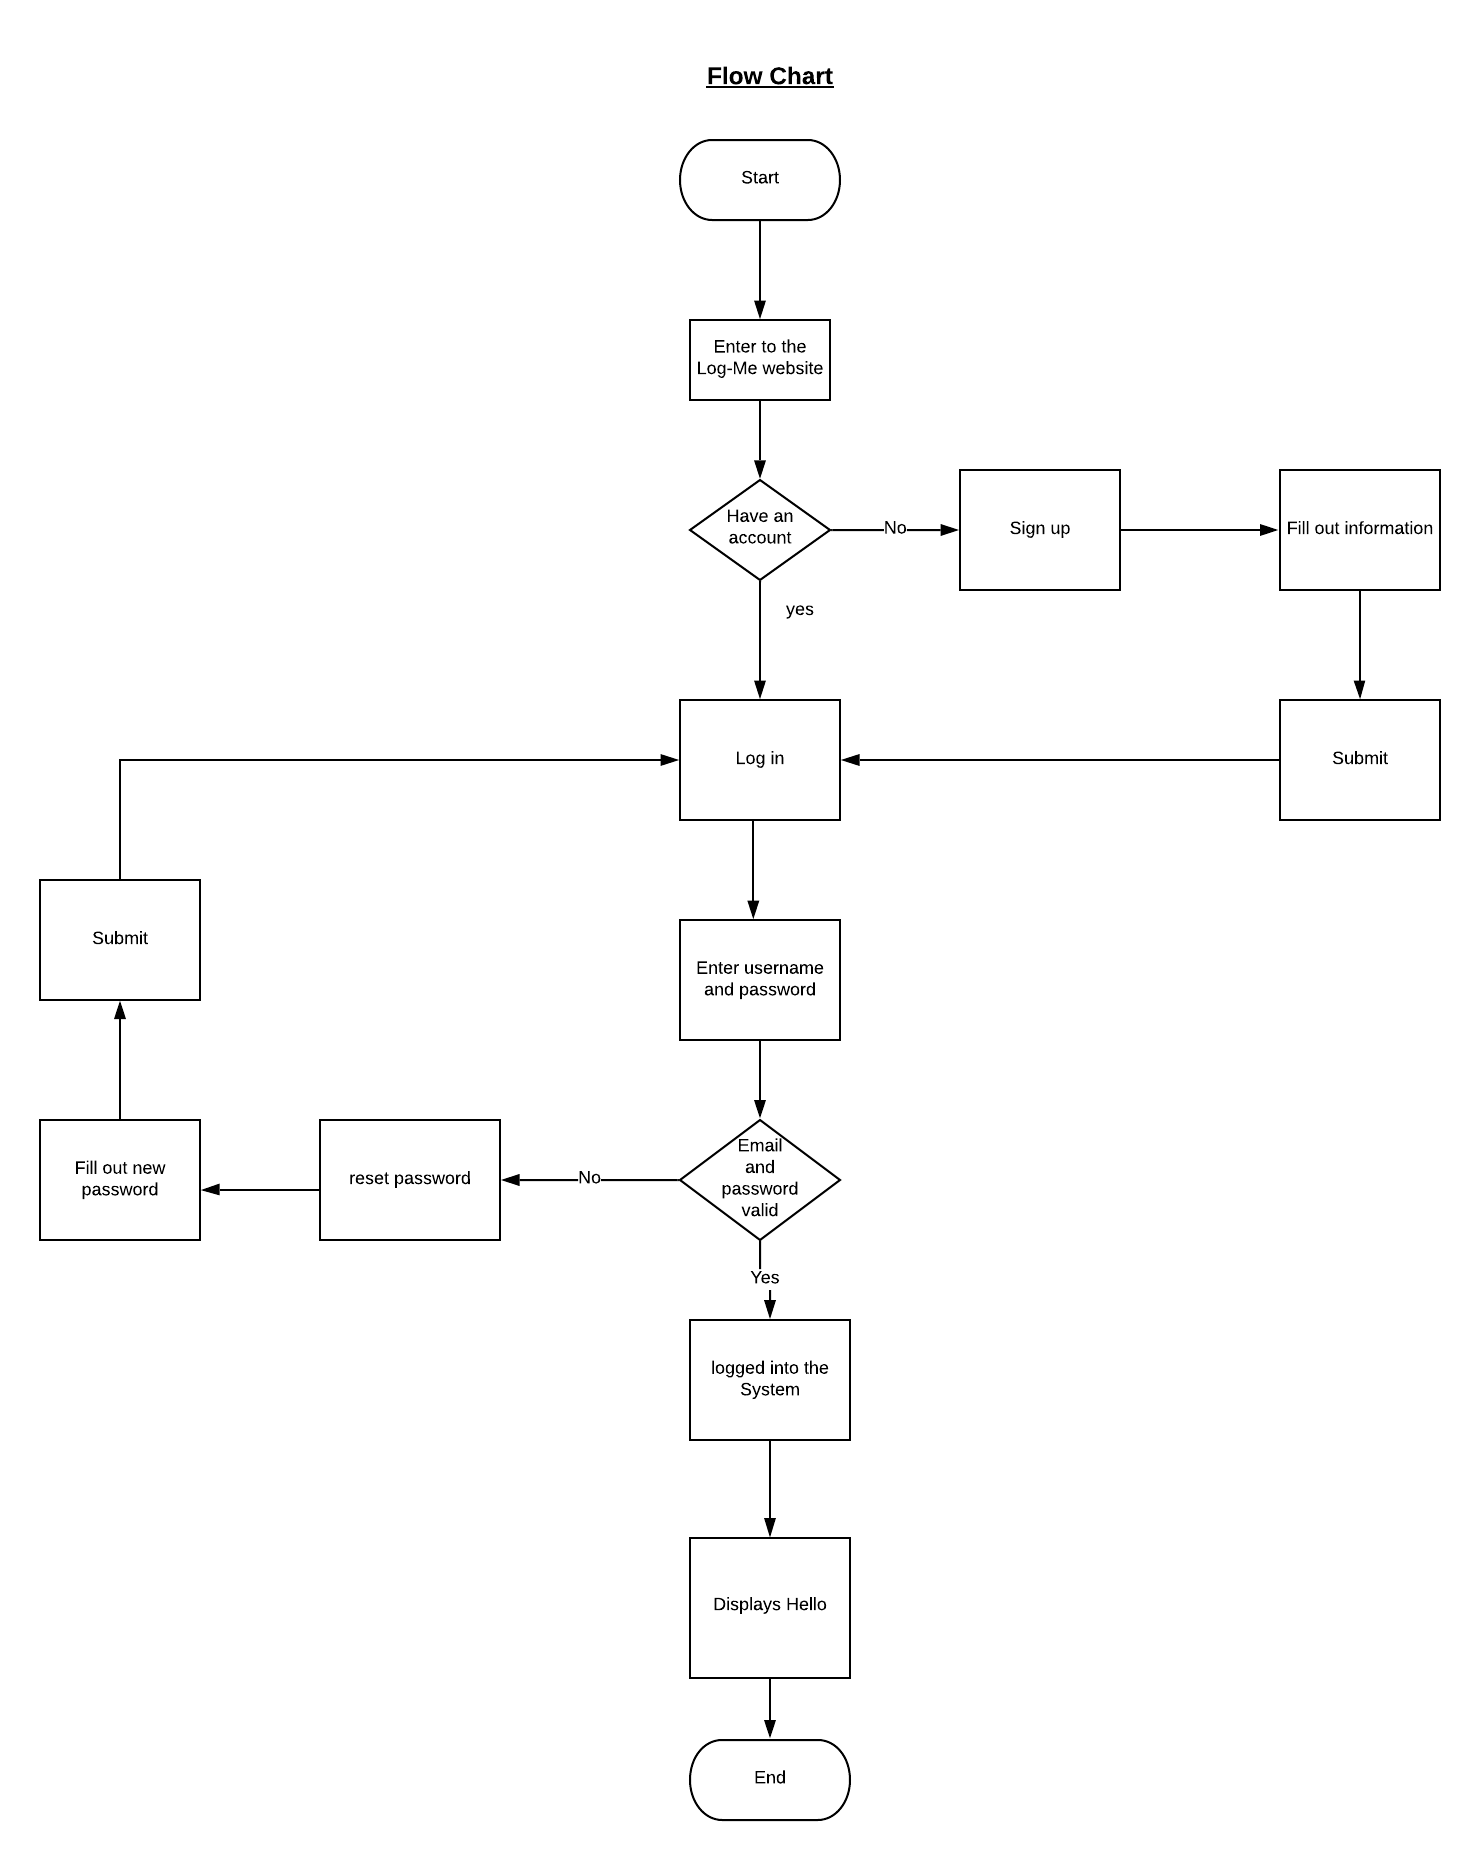
\includegraphics[width=100mm,scale=7.0]{Blank Diagram.png}
\end{center}






%uoooooooooooooooo tumadreuooooooooooooooooooo UOOOOOOOOOOOOOOOOOOOOOOOOOOOOOOOOOOOOOOOOO
%AL FIN SE TERMINA ESTA PUTA MIERDA!!!!
%USEGREAS OSTOJEOGIRN ojeogiek


\end{document}
